% =================================================================================================
% set document class
% =================================================================================================
\documentclass[mathserif,dvipsnames,table,xcdraw]{beamer}

% =================================================================================================
% packages
% =================================================================================================
\usepackage{animate}
\usepackage{multicol}
\usepackage{algorithm}
\usepackage{algpseudocode}
\usepackage{amsmath}
\usepackage{amssymb}
\usepackage{amsthm}
\usepackage{hyperref}
\usepackage{mathtools}
\usepackage{bm}
\usepackage[utf8]{inputenc}
\usepackage[english]{babel}
\usepackage[T1]{fontenc}
\usepackage{tcolorbox}
\usepackage{tikz}
\usepackage{tikz-3dplot}
\usepackage{pgfplots}
\usepackage{transparent}
\usepackage{calligra}
\usepackage{fancyvrb}
\usepackage{textcomp}
\RequirePackage{fix-cm}

% =================================================================================================
% libraries
% =================================================================================================
\usetikzlibrary{fadings,shapes.geometric,calc,intersections,through,decorations.shapes}
\usetikzlibrary{arrows.meta,patterns,snakes,backgrounds,fit,angles,quotes,graphs,trees}
\usetikzlibrary{decorations.pathmorphing,backgrounds,positioning,fit,petri,positioning}
\usetikzlibrary{spy,mindmap,shadows,automata,shapes.misc,babel,scopes,svg.path,animations,bending}

% =================================================================================================
% set mode and theme
% =================================================================================================
\mode<presentation>{\usetheme{Antibes}\usecolortheme{orchid}}

% =================================================================================================
% input definitions 
% =================================================================================================
%% math defs.tex
\newcommand{\ones}{\mathbf 1}
\newcommand{\reals}{{\mbox{\bf R}}}
\newcommand{\integers}{{\mbox{\bf Z}}}
\newcommand{\symm}{{\mbox{\bf S}}}  % symmetric matrices

\newcommand{\nullspace}{{\mathcal N}}
\newcommand{\range}{{\mathcal R}}
\newcommand{\Rank}{\mathop{\bf Rank}}
\newcommand{\Tr}{\mathop{\bf Tr}}
\newcommand{\diag}{\mathop{\bf diag}}
\newcommand{\card}{\mathop{\bf card}}
\newcommand{\rank}{\mathop{\bf rank}}
\newcommand{\conv}{\mathop{\bf conv}}
\newcommand{\prox}{\mathbf{prox}}

\newcommand{\Expect}{\mathop{\bf E{}}}
\newcommand{\Prob}{\mathop{\bf Prob}}
\newcommand{\Co}{{\mathop {\bf Co}}} % convex hull
\newcommand{\dist}{\mathop{\bf dist{}}}
\newcommand{\argmin}{\mathop{\rm argmin}}
\newcommand{\argmax}{\mathop{\rm argmax}}
\newcommand{\epi}{\mathop{\bf epi}} % epigraph
\newcommand{\Vol}{\mathop{\bf vol}}
\newcommand{\dom}{\mathop{\bf dom}} % domain
\newcommand{\intr}{\mathop{\bf int}}
\newcommand{\sign}{\mathop{\bf sign}}

\newcommand{\cf}{{\it cf.}}
\newcommand{\eg}{{\it e.g.}}
\newcommand{\ie}{{\it i.e.}}
\newcommand{\etc}{{\it etc.}}
%% define some colors (generated for Antibes)
\definecolor{PERSIAN_BLUE}{RGB}{51,51,178}
\definecolor{RAISIN_BLACK}{RGB}{42,45,52}
\definecolor{RUSSIAN_GREEN}{RGB}{92,148,110}
\definecolor{BLIZZARD_BLUE}{RGB}{160,221,230}
\definecolor{DARK_ORANGE}{RGB}{255,143,41}
\definecolor{PICOTEE_BLUE}{RGB}{38,38,134}
\definecolor{BISTRE}{RGB}{55,44,37}
\definecolor{GRAY_WEB}{RGB}{131,131,131}
\definecolor{DARK_SKY_BLUE}{RGB}{147,183,190}
\definecolor{MINT_CREAM_1}{RGB}{241,255,250}
\definecolor{MINT_CREAM_2}{RGB}{247,255,247}
\definecolor{PALE_SILVER}{RGB}{213,199,188}
\definecolor{OPAL}{RGB}{148,191,190}
\definecolor{LASER_LEMON}{RGB}{252,252,98}
\definecolor{MINDARO}{RGB}{218,255,125}
\definecolor{GRANNY_SMITH_APPLE}{RGB}{178,239,155}
\definecolor{RHYTHM}{RGB}{140,134,170}
\definecolor{SILVER}{RGB}{197,197,197}
\definecolor{SPANISH_GRAY_1}{RGB}{130,145,145}
\definecolor{SPANISH_GRAY_2}{RGB}{148,155,150}
\definecolor{BRICK_RED}{RGB}{195,60,84}
\definecolor{SKY_BLUE_CRAYOLA}{RGB}{142,227,239}
\definecolor{CELESTE}{RGB}{174,243,231}
\definecolor{HOOKERS_GREEN}{RGB}{88,125,113}
\definecolor{GREEN_PANTONE}{RGB}{77,170,87}
\definecolor{NAPLES_YELLOW}{RGB}{255,130,109}
\definecolor{AIR_SUPERIORITY_BLUE}{RGB}{108,166,193}
\definecolor{FIRE_BRICK}{RGB}{179,0,27}
\definecolor{ICE_BERG}{RGB}{126,163,204}
\definecolor{TAN}{RGB}{204,173,143}
\definecolor{MIDDLE_BLUE}{RGB}{247,255,247}
\definecolor{LAVENDER_BLUSH}{RGB}{238,229,233}
\definecolor{CINNABAR}{RGB}{214,73,51}
\definecolor{BABY_POWDER}{RGB}{247,247,242}
\definecolor{AQUA_MARINE}{RGB}{133,255,199}
\definecolor{CORAL}{RGB}{255,133,82}
\definecolor{PLATINUM}{RGB}{230,230,230}
\definecolor{BROWN}{RGB}{126,89,32}
\definecolor{FULVOUS}{RGB}{220,133,31}
\definecolor{YELLOW_ORANGE}{RGB}{255,167,55}
\definecolor{BITTER_SWEET}{RGB}{255,111,89}
\definecolor{ZOMP}{RGB}{67,170,139}
\definecolor{AMARANTH_RED}{RGB}{215,29,45}
\definecolor{SPACE_CADET}{RGB}{49,61,90}
\definecolor{CELADON_BLUE}{RGB}{66,129,164}
\definecolor{ELECTRIC_BLUE}{RGB}{142, 237, 247}
\definecolor{BABY_BLUE_EYES}{RGB}{161, 205, 241}
\definecolor{STAR_COMMAND}{RGB}{34, 116, 165}
\definecolor{DENIM_BLUE}{RGB}{57, 67, 183}
\definecolor{BLUE_JEANS}{RGB}{72, 172, 240}
\definecolor{UPSDELL_RED}{RGB}{180, 24, 37}
\definecolor{RED_MUNSELL}{RGB}{228, 58, 72}
\definecolor{BLUE_MUNSELL}{RGB}{27, 154, 170}
\definecolor{LIBERTY}{RGB}{76, 76, 157}
\definecolor{BABY_BLUE}{RGB}{108, 207, 246}
\definecolor{CAROLINA_BLUE}{RGB}{27, 152, 224}
\definecolor{MINION_YELLOW}{RGB}{242, 220, 93}
\definecolor{SANDY_BROWN}{RGB}{242, 163, 89}
\definecolor{FLAME}{RGB}{215, 78, 9}
\definecolor{BLOOD_RED}{RGB}{110, 14, 10}
\definecolor{CLARET}{RGB}{137, 4, 61}
\definecolor{EMERALD}{RGB}{68, 207, 108}
\definecolor{ILLUMINATING_EMERALD}{RGB}{50, 147, 111}
\definecolor{MAROON_X_11}{RGB}{184, 19, 101}
\definecolor{CARRIBEAN_GREEN}{RGB}{29, 211, 176}
\definecolor{RED_CRAYOLA}{RGB}{239, 45, 86}
\definecolor{EGG_SHELL}{RGB}{244, 236, 214}
\definecolor{AMAZON}{RGB}{74, 120, 86}
\definecolor{GOOGLE_G}{RGB}{60, 186, 84}
\definecolor{GOOGLE_Y}{RGB}{244, 194, 13}
\definecolor{GOOGLE_R}{RGB}{219, 50, 54}
\definecolor{GOOGLE_B}{RGB}{72, 133, 237}
\definecolor{PRINCETON_ORANGE}{RGB}{245, 128, 38}
\definecolor{YALE_BLUE}{RGB}{0, 68, 128}
\definecolor{MIKADO_YELLOW}{RGB}{255, 193, 0}
\definecolor{SELECTIVE_YELLOW}{RGB}{255, 186, 8}
\definecolor{MISTY_ROSE}{RGB}{255, 227, 220}
\definecolor{HONEY_YELLOW}{RGB}{247, 179, 43}
\definecolor{RUBY_RED}{RGB}{154, 3, 30}
\definecolor{BRONZE}{RGB}{203, 121, 58}
\definecolor{CELADON}{RGB}{172,247,193}
\definecolor{GREEN_SHEEN}{RGB}{128,194,175}
\definecolor{CITRINE}{RGB}{224, 202, 60}
\definecolor{MELLOW_APRICOT}{RGB}{255, 184, 111}
\definecolor{GLOSSY_GRAPE}{RGB}{171,146,191}
\definecolor{PINK_LAVENDER}{RGB}{212, 178, 216}
\definecolor{MAGIC_MINT}{RGB}{139, 232, 203}
\definecolor{MANATEE}{RGB}{141, 153, 174}
\definecolor{ALICE_BLUE}{RGB}{237, 242, 244}
\definecolor{SPANISH_BISTRE}{RGB}{111, 115, 47}
\definecolor{CAMEL}{RGB}{179, 138, 88}
\definecolor{PORTLAND_ORANGE}{RGB}{244, 96, 54}
\definecolor{PERSIAN_GREEN}{RGB}{27, 153, 139}
\definecolor{BEIGE}{RGB}{235, 235, 211}
\definecolor{CERISE}{RGB}{218, 65, 103}
\definecolor{LAVENDER_BLUE}{RGB}{183, 195, 243}
\definecolor{CYCLAMEN}{RGB}{221, 117, 150}
\definecolor{POPSTAR}{RGB}{175, 93, 99}
\definecolor{FERN_GREEN}{RGB}{91, 117, 83}




% =================================================================================================
% new command definitions 
% =================================================================================================
\newcommand{\fnt}[1]{\fontsize{#1}{0}\selectfont}
\newcommand{\tz}{Ti\textit{k}Z}
\newcommand{\tzrm}{\textrm{\tz}}
\newcommand{\redaccent}[1]{\textcolor{CERISE}{#1}}

% =================================================================================================
% title
% =================================================================================================
\title[Short tutorial on \tz]{
	Short tutorial on \tz 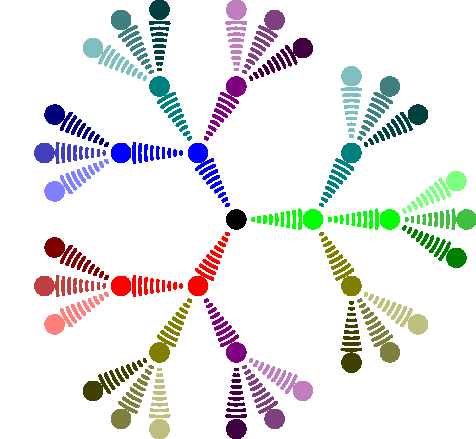
\includegraphics[width=0.1\textwidth]{../figures/tikz_tree.pdf}
}
\subtitle{Drawing with exact precision}
\author{\textcolor{RAISIN_BLACK}{Pritam Karmokar}}
\institute{
	% \textcolor{RUSSIAN_GREEN}{\textbf{}} \newline \newline
	% \textcolor{RUBY_RED}{Robotic Vision Lab (RVL)}\newline 
	\textcolor{LAVENDER_BLUE}{[Weekly Meeting 03/12/2021]}
}
\date{}

\titlegraphic{\hfill 
\includegraphics[height=0.8cm]{../figures/rvl_full_logo.pdf}}

% =================================================================================================
% document
% =================================================================================================
\begin{document}

% -------------------------------------------------------------------------------------------------
% title 
% -------------------------------------------------------------------------------------------------
%% title frame
\begin{frame}
	\titlepage
\end{frame}

% -------------------------------------------------------------------------------------------------
% table of contents 
% -------------------------------------------------------------------------------------------------
%% ToC
\begin{frame}{Table of Contents}
	\tableofcontents
\end{frame}

%% ToC at beginning of sections
\AtBeginSection[]
{
\begin{frame}{Table of Contents}
	\tableofcontents[currentsection]
\end{frame}
}

%% ToC at beginning of subsections
\AtBeginSubsection[]
{
\begin{frame}{Table of Contents}
	\tableofcontents[currentsubsection]
\end{frame}
}


% -------------------------------------------------------------------------------------------------
% introduction 
% -------------------------------------------------------------------------------------------------
\section[Introduction to \tz]{Introduction}
\label{sec:introduction}

\begin{frame}{What is \tz?}
	\begin{block}{\tz ...}
		\begin{itemize}
			\item <2-> ...is a recursive acronym for "\redaccent{T}i\textit{k}Z \textit{\redaccent{i}st \redaccent{k}ein \redaccent{Z}eichenprogramm}"
			\item <3-> is probably the most complex and powerful tool for creating graphic elements in \LaTeX
			\item <4-> defines a number of \TeX\ commands that draw graphics
		\end{itemize}
	\end{block}
\end{frame}

\begin{frame}{Good and Bad 
\includegraphics[width=2ex]{../figures/yin_yang.pdf}}
	Pros:
	\begin{itemize}
		\item<1-> Quick creation of simple graphics
		\item<2-> Drawing programmatically with exact precision
		\item<3-> Superior consistent typography
	\end{itemize}
	\only<4->{Cons:}
	\begin{itemize}
		\item<4-> Steep learning curve
		\item<5-> No WYSIWYG
		\item<6-> Changes require recompilation
	\end{itemize}
\end{frame}

\begin{frame}[fragile]\frametitle{Quick examples}
	\begin{example}[line]
		\begin{verbatim}
			\tikz \draw (0pt,0pt) -- (20pt,6pt);
		\end{verbatim}
		yields \tikz \draw (0pt,0pt) -- (20pt,6pt);
	\end{example}
	\begin{example}[orange]<2->
		\begin{verbatim}
			\tikz \fill[orange] (1ex,1ex) circle (1ex);
		\end{verbatim}
		yields \tikz \fill[orange] (1ex,1ex) circle (1ex);
	\end{example}
\end{frame}

\begin{frame}{Practical examples}
	\begin{columns}
		\column{0.5\textwidth}
			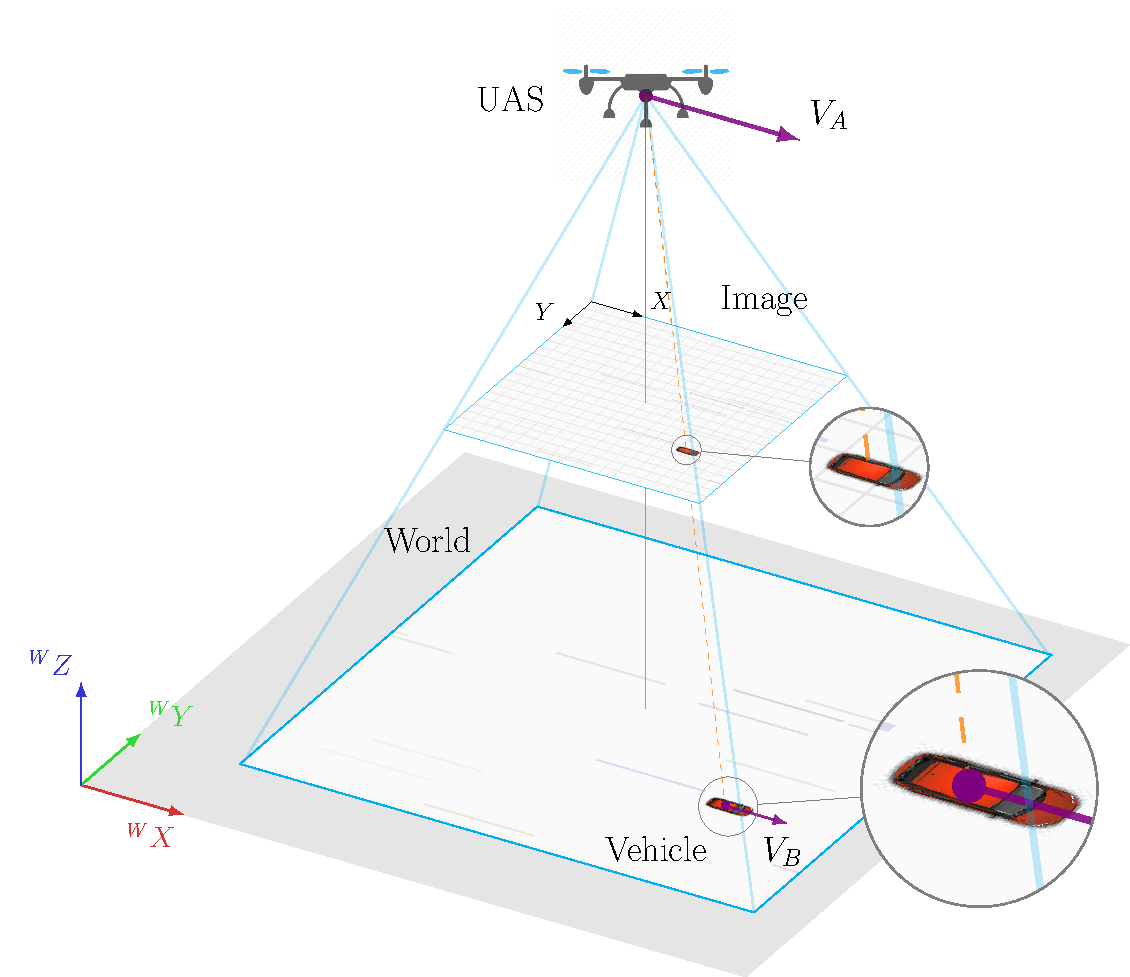
\includegraphics[width=\textwidth]{../figures/intro.pdf}
		\column{0.5\textwidth}
			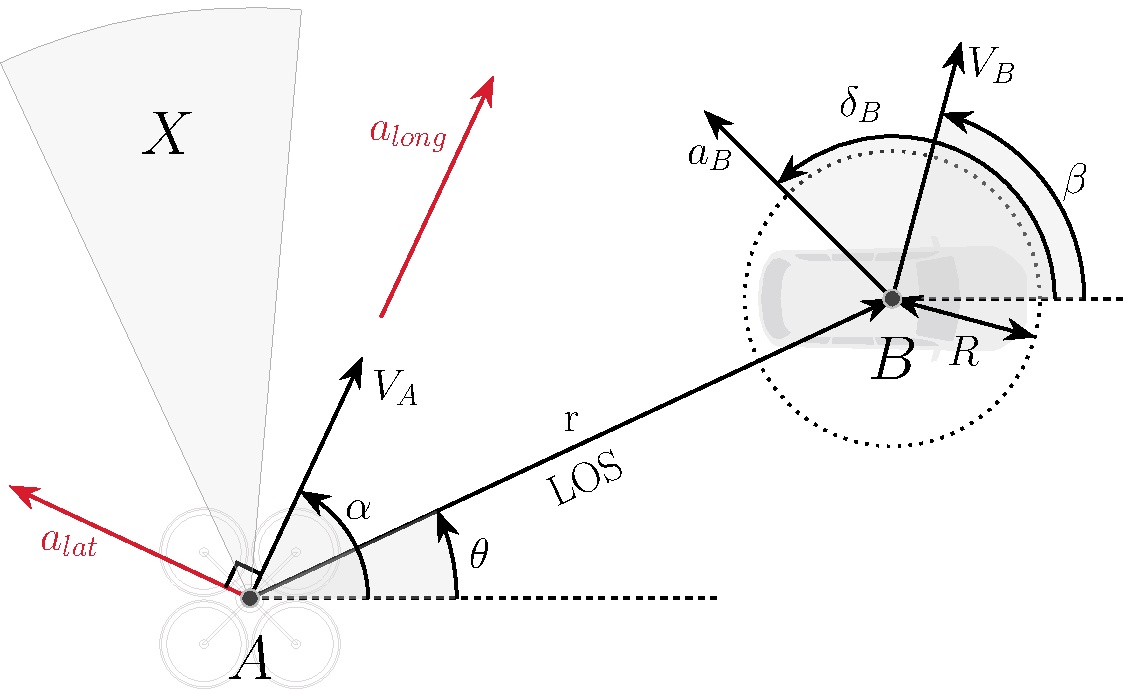
\includegraphics[width=0.8\textwidth]{../figures/engagement_geom.pdf}
	\end{columns}
\end{frame}


% -------------------------------------------------------------------------------------------------
% the basics
% -------------------------------------------------------------------------------------------------
\section[The Basics]{The Basics}
\label{sec:the_basics}

\begin{frame}[fragile]\frametitle{Hello, \tz!}
	\texttt{\textbackslash begin\{\textcolor{RED_CRAYOLA}{tikzpicture}\}\textcolor{EMERALD}{\textlangle{}\textit{animations spec}\textrangle{}[\textlangle{}\textit{options}\textrangle{}]}\\
	\hspace{4ex}\textlangle{}\textit{environment contents}\textrangle{}\\
	\textbackslash end\{\textcolor{RED_CRAYOLA}{tikzpicture}\}
	}
	\begin{example}<2->[tikzpicture]
	\begin{verbatim}
		\usepackage{tikzpicture}  %preamble
		...
		\begin{document}
		    \begin{tikzpicture}
		        \path[draw] (0pt,0pt) -- (20pt,6pt);
		    \end{tikzpicture}
		\end{document}
	\end{verbatim}
	\end{example}
\end{frame}


\subsection[Basic Design Principles]{Basic Design Principles}
\label{subsec:basic_design_principles}

\begin{frame}{Basic Design Principles}
	\begin{multicols}{2}
		\begin{enumerate}
			\item<1-> Special syntax for specifying points
			\item<1-> Special syntax for path specifications
			\item<2-> Actions on paths
			\item<3-> Key-value syntax for graphic parameters
			\item<4-> Special syntax for nodes
			\item<4-> Special syntax for trees
			\item<4-> Special syntax for graphs
			\item<5-> Grouping of graphic parameters
			\item<6-> Coordinate transformation system
		\end{enumerate}
	\end{multicols}
\end{frame}

\begin{frame}{Special syntax for specifying points}
	\begin{itemize}
		\item<1-> Cartesian: \texttt{(1cm,2pt)} or Polar: \texttt{(30:1cm)}
		\item<1-> Default units: length - centimeters (cm),  angle - degrees (${}^{\circ}$)
		\item<2-> 3D xyz-coordinate: \texttt{(1,2,3)}
		\item<3-> Anchor as coordinate: \texttt{(mynode\_1 node.south)}
		\item<4-> Relative coordinates \textit{(1) change current point (2) don't change }
		\begin{enumerate}
			\item \texttt{(1,0), ++(1,0), ++(0,1)} would specify \texttt{(1,0)}, then \texttt{(2,0)}, and \texttt{(2,1)}
			\item \texttt{(1,0), +(1,0), +(0,1)} would specify \texttt{(1,0)}, then \texttt{(2,0)}, and \texttt{(1,1)}
		\end{enumerate}
	\end{itemize}
\end{frame}

\begin{frame}[fragile]\frametitle{Special syntax for path specifications}
	\begin{itemize}
		\item<1-> A \textit{path} is a series of straight or curved lines, which need not be connected
		\item<2-> Path specification is the main part while creating \tz\ pictures
	\end{itemize}
	\begin{example}<3->[\textit{path} specification]
		\begin{verbatim}
			\tikz{\filldraw[fill=white,draw=red,] 
			        (5pt,0pt)--(0pt,0pt)--(0pt,5pt)--cycle;}
		\end{verbatim}
		yields \tikz{\filldraw [fill=white,draw=red,]
					(5pt,0pt)--(0pt,0pt)--(0pt,5pt)--cycle;}
	\end{example}
\end{frame}

\begin{frame}{Actions on paths}
	\begin{itemize}
		\item<1-> A \textit{path} is a series of straight or curved lines, which need not be connected
		\item<2-> We need to specify what needs to happen with it
		\item<3-> \textit{draw}, \textit{fill}, \textit{shade}, \textit{clip} or a combination?
		\item<4-> \texttt{\textbackslash draw} is shorthand for \texttt{\textbackslash path[draw]}
		\item<5-> Likewise, \texttt{\textbackslash fill}, \texttt{\textbackslash shade}, \texttt{\textbackslash clip}
	\end{itemize}
\end{frame}

\begin{frame}[fragile]\frametitle{Key-value syntax for graphic parameters}
	\begin{example}[Key-value]
		\begin{verbatim}
			\tikz{
				    \draw[
			            line width=2pt,color=red,
			            densely dotted,rounded corners,
			    	    ] 
			            (1,0) -- (0,0) -- (0,1) -- cycle;
			    }
		\end{verbatim}
		yields \tikz{\draw[line width=2pt,color=red,densely dotted,rounded corners] 
		(1,0)--(0,0)--(0,1)--cycle;}
	\end{example}
\end{frame}

\begin{frame}[fragile]\frametitle{Special syntax for nodes}
	\begin{example}[nodes]
		\begin{verbatim}
			\tikz{
			    \draw[darkgray,very thick] 
			    (1,1)
			    node[circle,draw=red] (dummytextnode)
			    {\textcolor{orange}{text}}
			    -- (2,2);
			}
		\end{verbatim}
		yields \tikz \draw[darkgray,very thick] (1,1) node[circle,draw=red] (dummytextnode) {\textcolor{orange}{text}} -- (2,2);
	\end{example}
\end{frame}

\begin{frame}[fragile]\frametitle{Special syntax for trees}
	\begin{example}[trees]
		\begin{multicols}{2}
		\begin{verbatim}
			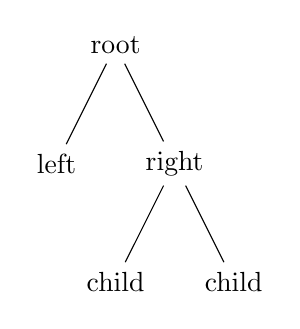
\begin{tikzpicture}
			    \node {root}
			    child {node {left}}
			    child {node {right}
			        child {node {child}}
			        child {node {child}}
			    };
			\end{tikzpicture}
		\end{verbatim}
		yields\\
		\centering
		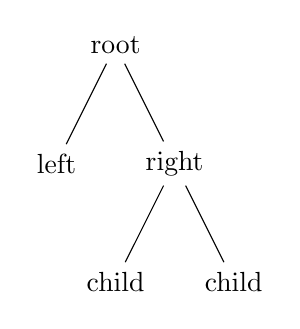
\begin{tikzpicture}
			\node {root}
			child {node {left}}
			child {node {right}
			child {node {child}}
			child {node {child}}
			};
		\end{tikzpicture}
		\end{multicols}
	\end{example}
\end{frame}

\begin{frame}[fragile]\frametitle{Special syntax for graphs}
	\begin{example}[graphs]
		\begin{multicols}{2}
		\begin{verbatim}
			\usetikzlibrary {graphs}
			\tikz
			    \graph[
			        grow down,
			        branch right] {
		    root->{left,
			        right->{child,
			            child}}};
		\end{verbatim}

		yields\\
		\centering
		\usetikzlibrary {graphs}
		\tikz \graph [grow down, branch right] {
		root -> { left, right -> {child, child} }
		};
	\end{multicols}
	\end{example}
\end{frame}

\begin{frame}[fragile]\frametitle{Grouping of graphic parameters}
	\begin{example}[grouping graphic parameters]
		\begin{multicols}{2}
		\begin{verbatim}
			
\begin{tikzpicture}
				\begin{scope}[red]
				\draw[ultra thick]
				    (0mm,8mm)--(10mm,8mm);
				\end{scope}
				\begin{scope}[green]
				\draw[ultra thick]
				    (0mm,4mm)--(10mm,4mm);
				\draw[blue,ultra thick]
				    (0mm,0mm)--(10mm,0mm);
				\end{scope}
				\end{tikzpicture}
		\end{verbatim}
		yields\\
		\centering
		
\begin{tikzpicture}
			\begin{scope}[red]
			\draw[ultra thick] (0mm, 8mm) -- (10mm, 8mm);
			\end{scope}
			\begin{scope}[green]
			\draw[ultra thick] (0mm, 4mm) -- (10mm, 4mm);
			\draw[blue,ultra thick] (0mm, 0mm) -- (10mm, 0mm);
			\end{scope}
			\end{tikzpicture}
		\end{multicols}
	\end{example}
\end{frame}

\begin{frame}[fragile]\frametitle{Coordinate transformation system}
	\begin{example}[coordinate transformation]
		\begin{multicols}{2}
		\begin{verbatim}
			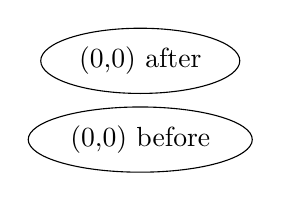
\begin{tikzpicture}
			    \node[ellipse,draw]
				    at (0,0) {(0,0) before};
			    \tikzset{yshift=10mm}
			    \node[ellipse,draw]
				    at (0,0) {(0,0) after};
			\end{tikzpicture}
		\end{verbatim}
		\vspace{3ex}
		yields\\
		\centering
		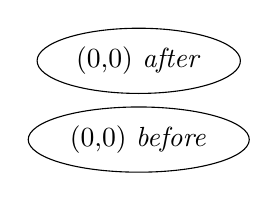
\begin{tikzpicture}
			\node[ellipse,draw] at (0,0) {(0,0) \textit{before}};
			\tikzset{yshift=10mm}
			\node[ellipse,draw] at (0,0) {(0,0) \textit{after}};
		\end{tikzpicture}
		\end{multicols}
	\end{example}
\end{frame}

\subsection[Simple exercise]{Simple exercise}
\label{subsec:simple_exercise}

\begin{frame}[fragile]\frametitle{Getting acquainted}
	\begin{block}{How could we draw this?}
		\centering{
		
\includegraphics[width=0.3\textwidth]{../figures/RVL_logo.png}}
		\begin{itemize}
			\item A triangle, an incircle and an inner circle
		\end{itemize}
	\end{block}
\end{frame}

\begin{frame}[fragile]\frametitle{Getting acquainted}
	\begin{block}{Break down}
		\centering{
		
\includegraphics[width=0.3\textwidth]{../figures/RVL_logo.png}}
		\begin{itemize}
			\item Triangle can be created by \textit{filling} through it's three coords
			\item Circles can be created readily by \textit{filling circles} at the \textit{incenter} coordinate 
		\end{itemize}
	\end{block}
\end{frame}

\begin{frame}[fragile]\frametitle{Getting acquainted}
	\begin{block}{Walk through}
		\begin{columns}
			\column{0.6\textwidth}
			\begin{verbatim}
			    \coordinate (A) at (0,0);
			    \coordinate (B) at (0,1cm);
			    \coordinate (C) at (60:1cm);
			    \coordinate (I) at (5mm,{1*sqrt(3)/6});
			\end{verbatim}
			\column{0.4\textwidth}
			\centering
			\hspace{3ex} 
\includegraphics[width=0.3\textwidth]{../figures/RVL_logo.png}
		\end{columns}
	\end{block}
\end{frame}

\begin{frame}[fragile]\frametitle{Getting acquainted}
	\begin{block}{Wrapping up}
		\begin{verbatim}
		\definecolor{YALE_BLUE}{RGB}{0, 68, 128}
		\definecolor{PRINCETON_ORANGE}{RGB}{245, 128, 38}

		\filldraw[fill=YALE_BLUE,draw=none] 
		    (A) -- (B) -- (C) -- cycle;
		\node[circle,minimum size={sqrt(3)/3},
		    fill=PRINCETON_ORANGE,draw=none,] at (I) {};
		\node[circle,minimum size={(1.25/pi)*sqrt(3)/6},
		    fill=YALE_BLUE,draw=none,] at (I) {};
		\end{verbatim}
	\end{block}
\end{frame}

\begin{frame}{Getting acquainted}
	\only<1>{
		The outcome\\ \vspace{3ex}
		\centering
		
\includegraphics[height=0.3\textwidth]{../figures/rvl_short_logo.pdf}
	}
	\only<2->{
		The outcome...\\ \vspace{3ex}
		\centering
		
\includegraphics[height=0.3\textwidth]{../figures/rvl_full_logo.pdf}
	}
\end{frame}

% -------------------------------------------------------------------------------------------------
% pgfplots
% -------------------------------------------------------------------------------------------------
\section[PGFPLOTS]{PGFPLOTS}
\label{sec:pgfplots}

\begin{frame}{Hello, PGFPLOTS!}
	{\redaccent{P}ortable \redaccent{G}raphics \redaccent{F}ormat}
	\centering
	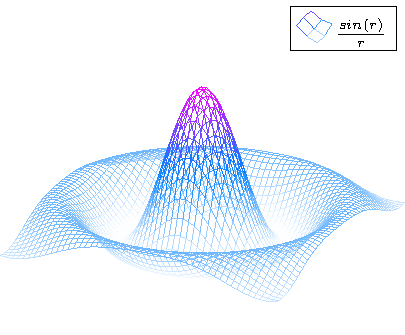
\includegraphics[width=0.7\paperwidth]{../figures/mesh_plot.pdf}
\end{frame}

\begin{frame}{Hello, PGFPLOTS!}
	\begin{itemize}
		\item<1-> PGFPLOTS is built completely on \tz/PGF
		\item<2-> Knowledge of \tz\ will simplify the work with PGFPLOTS
		\item<3-> PGFPLOTS comes with two components:
		\begin{enumerate}
			\item<4-> the plotting component
			\item<5-> PGFPLOTSTABLE component which simplifies number formatting and postprocessing of numerical
			tables. (separate package)
		\end{enumerate}
	\end{itemize}
\end{frame}


\begin{frame}[fragile]\frametitle{A quick intro}
	\begin{example}[code]
		\begin{verbatim}
			\begin{tikzpicture}
			    \begin{axis}[]
			        \addplot [
			            red,
			            domain=-3e-3:3e-3,
			            samples=201,
			        ]
			        {exp(-x^2 / (2e-3^2)) / (1e-3 * sqrt(2*pi))};
			    \end{axis}
			\end{tikzpicture}
		\end{verbatim}
		
	\end{example}
\end{frame}

\begin{frame}[fragile]\frametitle{A quick intro}
	\begin{example}[output]	
		\centering
		\begin{tikzpicture}[scale=0.9]
			\begin{axis}[
			]
			% density of Normal distribution:
			\addplot [
			red,
			domain=-3e-3:3e-3,
			samples=201,
			]
			{exp(-x^2 / (2e-3^2)) / (1e-3 * sqrt(2*pi))};
			\end{axis}
			\end{tikzpicture}
	\end{example}
\end{frame}

\begin{frame}{In practice}
	\centering
	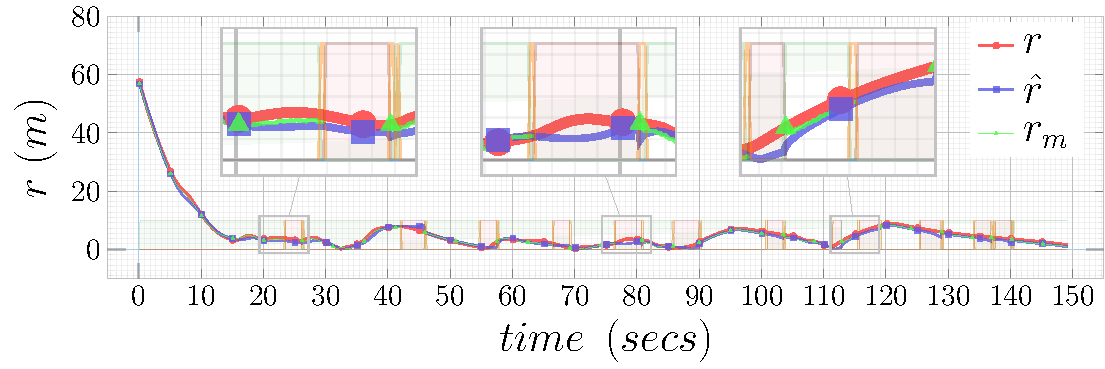
\includegraphics[width=0.9\textwidth]{../figures/plot_los_1.pdf}\\
	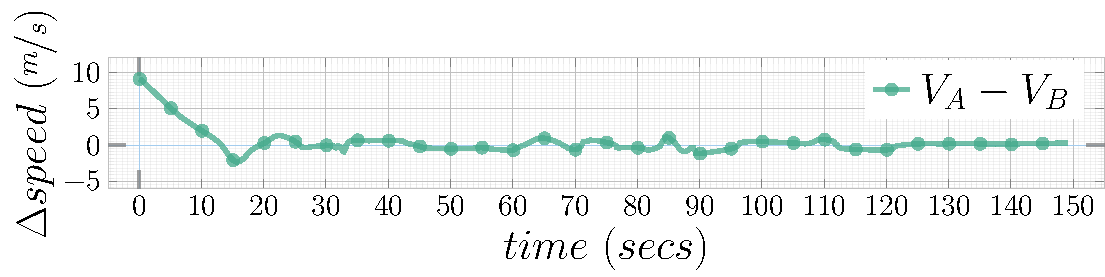
\includegraphics[width=0.9\textwidth]{../figures/plot_speed_diff.pdf}
\end{frame}

\begin{frame}{In practice}
	\centering
	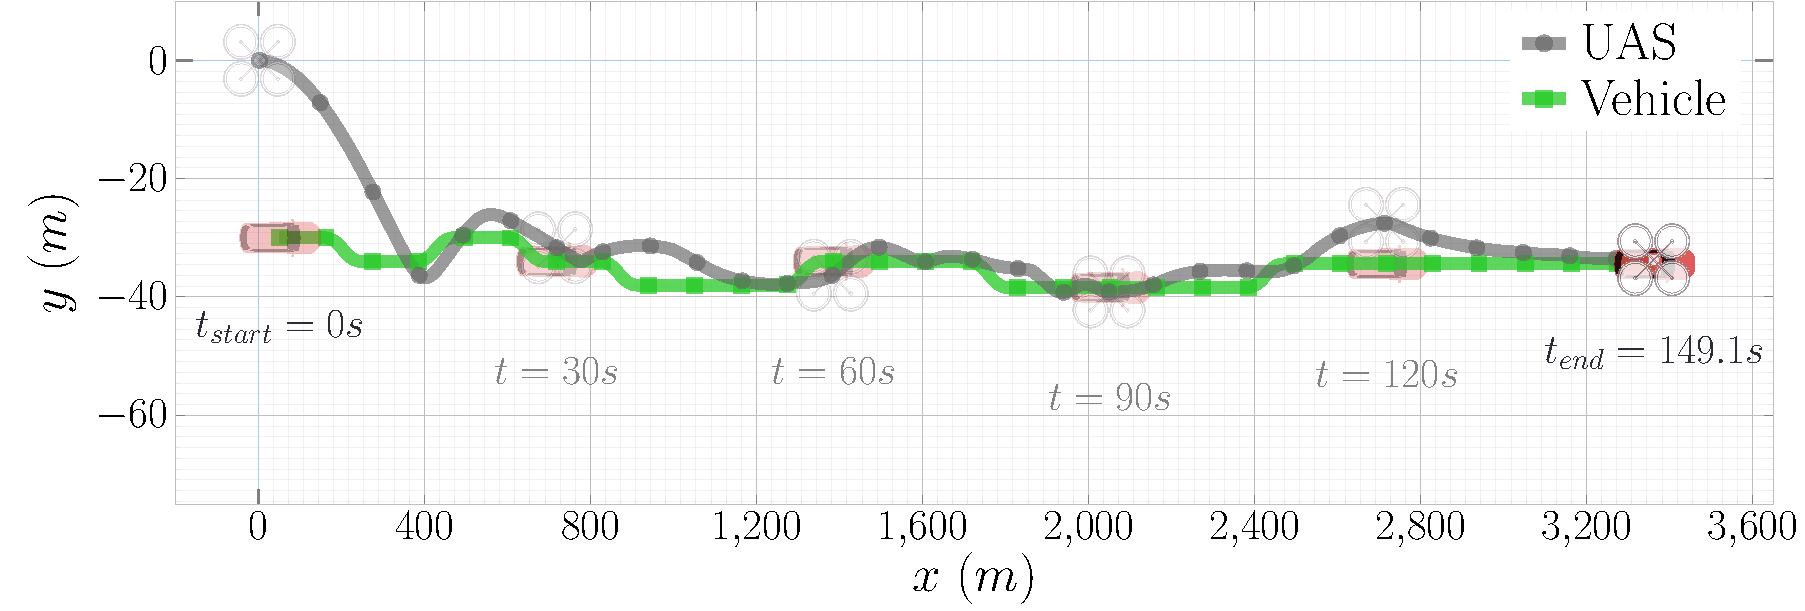
\includegraphics[width=\textwidth]{../figures/plot_traj_world.pdf}
\end{frame}

\begin{frame}{That's all folks!}
	Some useful resources
	\begin{itemize}
	\item \href{https://stuff.mit.edu/afs/athena/contrib/tex-contrib/beamer/pgf-1.01/doc/generic/pgf/version-for-tex4ht/en/pgfmanual.html\#pgfmanualse10.html}{Online \tz /PGF web manual}
	\item \href{https://www.overleaf.com/learn/latex/TikZ_package}{Overleaf \tz\ doc}
	\item \href{https://mavsuta-my.sharepoint.com/:f:/r/personal/william_beksi_uta_edu/Documents/Research/Robotic\%20Vision\%20Laboratory/Presentations/2021/TikZ/TikZ\%20docs?csf=1&web=1&e=4cLrLa}{RVL archives}
	\item \href{https://tex.stackexchange.com/questions/158668/nice-scientific-pictures-show-off}{Scientific pictures show off}
	\item \href{https://awesomerepos.io/awesome/xiaohanyu/awesome-tikz}{Awesome \tz\ repos}
	\end{itemize}
\end{frame}

% -------------------------------------------------------------------------------------------------
% conclusion
% -------------------------------------------------------------------------------------------------
\section{Conclusion}
\label{sec:conclusion}

	\begin{frame}{To be continued..}
		Summary
		\begin{itemize}
			\item \tz\ is cryptic, painful but an awesome drawing package
			\item Like some other skills it will need constant touch
			\item PGFPLOTS and PGFPLOTSTABLE can aid our process of making quality illustrative figures and tables in research papers
		\end{itemize}
		
	\end{frame}


% -------------------------------------------------------------------------------------------------
% extro
% -------------------------------------------------------------------------------------------------
	\begin{frame}{Thank you}
		\centering
		\textcolor{RAISIN_BLACK}{\Huge\calligra Fin.}
	\end{frame}

\end{document}

